% !TEX root = ../Thesis.tex

%beschrijving van het opgeleverde eindproduct, plusminus 15 pagina’s
\section{Design \& Implementation}
\label{sec:design-implementation} 
In this section, we depict the high-level architecture of the parser.
We do this by first giving an architecture overview in \autoref{design:system-overview}.
Then we elaborate on the code quality in \autoref{design:software-quality}.
The new lexer is described in \autoref{design:lexer} and \autoref{design:new-lexer}, while the parser itself is depicted in \autoref{design:new-parser}.
Finally, improved error messages are covered in \autoref{design:errors}.
The new test suite is described later in \autoref{sec:tests} and additional more detailed artifacts are given in the project documentation \citepr{documentation}.

% !TEX root = ../Documentation.tex

\subsection{System overview}
\label{design:system-overview}
  The parser module overview is given in \autoref{fig:ParserModules}.
  \begin{figure}[ht]%
    \centering
    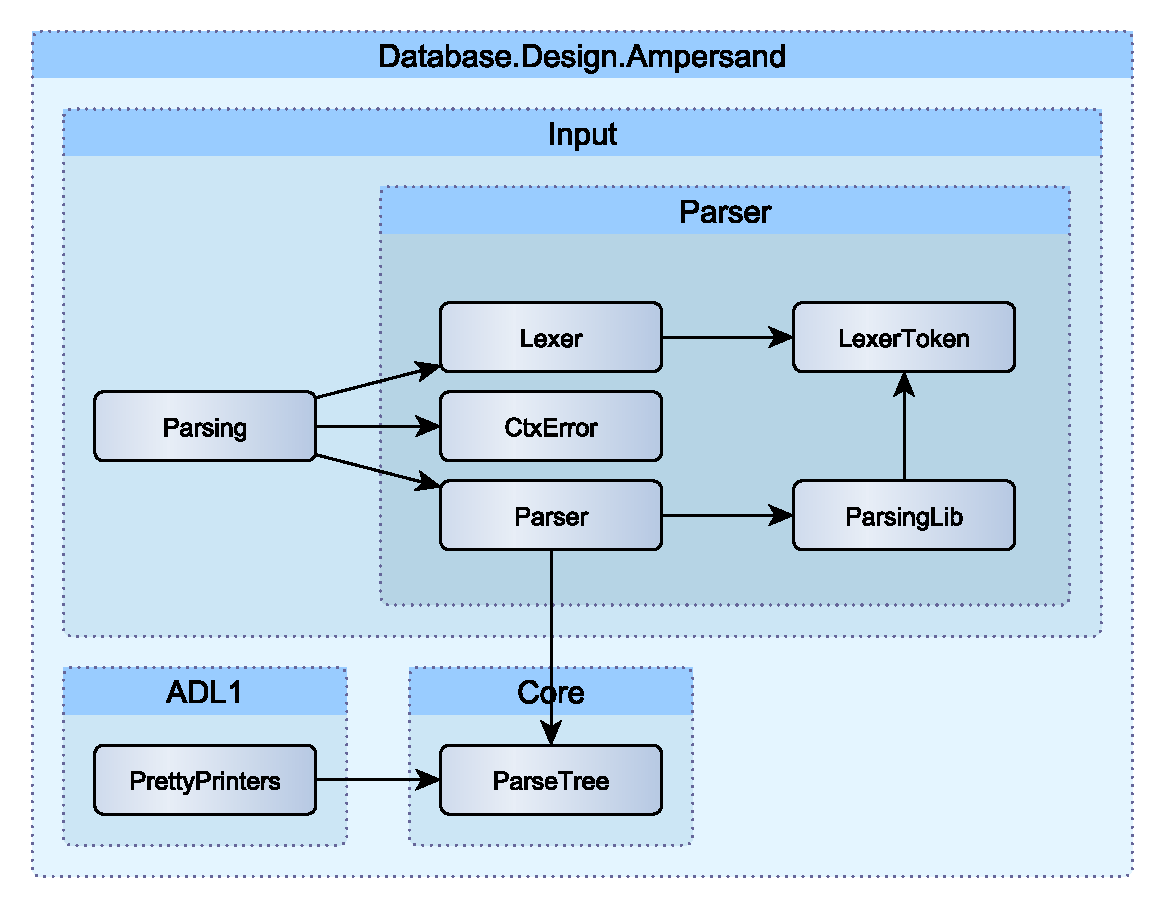
\includegraphics[width=0.7\columnwidth]{Figures/ParserModules}
    \caption{The modules relevant for the parser and their dependencies}
    \label{fig:ParserModules}
  \end{figure}%

  The parsing process starts in the module \code{Parsing}.
  As a first step, the input string is sliced into tokens by the \code{lexer} module.
  Once the input string is separated into the token structure as defined in the module \code{LexerToken} the next step is to actually parse the tokens by the \code{Parser}.
  The parser will use the \code{ParsingLib} to create the parse tree as defined in \code{ParseTree}.

  ~\\\noindent
  Each main module has the following responsibilities:
  %
  \begin{description}
    \item[Parsing] module that implements the interface of the parser with the rest of the system.
      It is responsible for reading the input files, calling the lexer and the parser and returning a parse tree as result (or a parse error).

    \item[Lexer/LexerToken] modules responsible for recognizing the input characters and converting them to tokens.
      The new lexer, together with its sub-modules, splits the input strings into the token structure defined in \code{LexerToken}.
      This list of tokens is the actual input for the parser.

    \item[Parser] module responsible for executing the parsing itself.
      It accepts the tokens that are allowed in each grammar production and generates the corresponding parse tree.
      The parser is described in \autoref{design:new-parser}.
 \end{description}

  \noindent
  Several supporting modules are defined used by one or more main modules:
  \begin{description}
    \item[ParsingLib] library that contains several useful functions to assist the parser, e.g. token recognition.
      These functions are not depending on the specific grammar rules.
      
    \item[ParseTree] external module containing the parse tree data structures.
      Only details of this module have been changed during this project (e.g. field ordering).
    
    \item[PrettyPrinters] contains instances of the \code{Pretty} type class for the parse tree data types and the functions responsible for printing the parse tree to ADL scripts in a `pretty' way.

    \item[CtxError] contains the data structures responsible for the parse errors and their location.
      This module has not been refactored as a part of this project.
    
  \end{description}

% !TEX root = ../Thesis.tex

\subsection{Sofware Quality Factors (M)}
\label{results:software-quality}
% Maintainability

\subsubsection{Documentation}
\lipsum[2]
% Haddock + EBNF comments

\subsubsection{Readability}
\lipsum[4]
% HLint + Shorter code + refactorings

\subsubsection{Performance}
\lipsum[5]
% Efficiency
% !TEX root = ../Thesis.tex

\subsection{New Lexer: The rationale behind the new lexer}
\label{subsec:newlexer}

In the design of the new Ampersand parser, the question arose whether to keep the current scanner, the former name of the lexer module within Ampersand, or to implement a new one.
After the analysis of the error improvement areas, as described in \autoref{sec:analysis}, the main improvements were identified within the actual parser.
The error feedback quality produced by the scanner module was higher and therefore, there was no stringent need to re-implement the scanner.
On the other hand, given the aspect that Parsec was defined as the new parser library, keeping the current scanner would have resulted in the utilization of two different libraries providing more of less the same functionality.
To avoid a decrease in maintainability, the decision is made to implement the parser and scanner based on the same library.

During the implementation of the lexer module, replacing the old scanner, additional attention was given to further improve the quality of the error messages.
The scanner module is renamed to lexer to stress the aspect that the principle of lexemes is used in the new scanner.
Lexemes can be seen as the part of a token containing the actual language content besides the actual position information.

The lexer is built based on the existing Helium lexer modules. 
Helium is a Haskell compiler with the main goal of giving user friendly error messages \citeac{helium}.
The lexer module in Helium contains interesting principles such as position monitoring, warnings and easy maintainable error messages.
% !TEX root = ../Thesis.tex

\subsection{Lexer}
\label{analysis:lexer}
The lexer module is responsible to split up the input stream into tokens.
Tokens are meaningful pieces of the input string that can be recognized by the parser.

The following improvement points were identified after analysis:
\begin{description}
  \item[Dispersed error messages]
    The error messages produced by the lexer are of good quality.
    Each error message is however defined directly within the corresponding lexer function making the maintenance harder.
  \item[Complex token structure]
    The token structure is complex and confusing.
    Two values are present in the token, of which one \texttt{val1} is never used.
    There is no distinction between the values used to identify the content of the token and the ones to determine the position of the token.
  \item[Module structuring]
    In the lexer, the actual lexing functions are intermingled with data types, supporting functions and error message texts.
    This makes the lexer hard to understand and to maintain.
  \item[Language support]
    The errors are returned in English only, no multilingual support is available.
  \item[No support for warnings]
    The lexer can only return errors, warnings are not supported. 
  \item[Strings only]
    Token values are stored as strings for all types, with no conversion of integer values.
  \item[Lacking documentation]
    There was no documentation available on how the lexer was designed and structured.
\end{description}


\subsubsection{Token structure}
The old token has the following structure:

\begin{verbatim}
data Token = Tok { tp' :: TokenType
                 , val1 :: String
                 , val2 :: String
                 , pos :: !Pos
                 , file :: !Filename
                 }

data TokenType
  = TkSymbol
  | TkVarid
  | TkConid
  | TkKeyword
  | TkOp
  | TkString
  | TkExpl
  | TkAtom
  | TkChar
  | TkInteger8
  | TkInteger10
  | TkInteger16
  | TkTextnm
  | TkTextln
  | TkSpace
  | TkError
  deriving (Eq, Ord)
\end{verbatim}
%
The arguments have the following purpose:
\begin{description}
  \item[TokenType]
    Identification of the token type. %, i.e. \texttt{TkSymbol}, \texttt{TkVarid}, \texttt{TkConid}, \texttt{TkKeyword}, \texttt{TkOp}, \texttt{TkString}, \texttt{TkExpl}, \texttt{TkAtom}, \texttt{TkChar}, \texttt{TkInteger8}, \texttt{TkInteger10}, \texttt{TkInteger16}, \texttt{TkTextnm}, \texttt{TkTextln}, \texttt{TkSpace} or \texttt{TkError}.
  \item[val1]
    This string argument is not used in the lexer.
    In the case of a \texttt{keyToken} creation, the value is filled in, but we could not find any purpose for this argument.
  \item[val2]
    The actual token content, stored as a string, including the integer values.
  \item[pos]
    Line and column number.
  \item[file]
     Filename in which the token is located.
\end{description}

% !TEX root = ../Thesis.tex

\subsection{New parser}
\label{design:new-parser}
The high-level design of the new parser has not changed much.
While the new parser may still be recognizable for the Ampersand developers, several improvements have been made.

As decided during the research for domain and techniques (see \autoref{domain:parsing}), the parser has been rebuilt with the Parsec combinator library.
Basically, each EBNF rule receives its own parser function.
Thanks to the combinator operators, each parsing function also looks very similar to its corresponding EBNF.

The applicative interface is consistently used.
By changing details of the implementation, e.g. the order of the fields in the parse tree, we have made many of the `rebuild' functions unnecessary.
For some parsers the amount of changes necessary in order to remove supporting functions was too large or even impossible with the current parse tree.

Note that in parts of the parser, the function syntax has substituted the record syntax for creating data objects.
This was done only when the code readability could be improved by doing so.

\subsubsection{Parsec}
\label{design:parsing-lib}
As mentioned earlier, and described in the research context document \citenac{parsing}, the new Ampersand parser has been rebuilt with another parsing library, namely Parsec.
However, for the Ampersand developers, the source code of the parser will still look very familiar, thanks to the applicative interface.
For developers, the main differences between Parsec and the uulib are:
\begin{itemize}
  \item Parsec does not backtrack by default.
    In order to enable backtracking, the \code{try} function must be used.
    This is described in \autoref{design:backtracking}.
  \item Parsec does not try to solve parsing errors.
    The parser stops immediately after the first issue.
   This way, the user is not overwhelmed with irrelevant information.
    See also the error analysis in \autoref{tests:errors}.
  \item Error messages are customizable by using the \code{<?>} operator.
    This is also suggested in \autoref{sec:recommendations}.
  \item Some combinators have a different name, e.g. one must use \code{option} instead of \code{opt}.
    Because the documentation found on Hackage is clear and sufficient, interface differences are not documented here.
\end{itemize}

\subsubsection{Backtracking}
\label{design:backtracking}
In order to explain the differences on backtracking behavior between the uulib and Parsec, we quote here Doaitse Swierstra, the author of the uulib \citenac{swierstra-parsec}:
\begin{quote}
\textsl{%
  To understand the subtleties it is important to understand the differences between the try construct in Haskell and the non-greedy parsing strategy used in uu-parsinglib.
  Effectively the latter is a try which just looks ahead one symbol.
  In that respect it is less powerful than the \code{try} construct from Parsec, in which you specify that a specific construct has to be present completely.
  And then there is the underlying different overall strategy.
  Parsec uses a back-tracking strategy with explicit tries to commit, whereas uu-parsinglib uses a breadth-first strategy with an occasional single symbol look-ahead.
}
\end{quote}
Although the \code{try} construct for backtracking in Parsec is very powerful, it is also undesirable:
Backtracking increases the parser's memory usage, speed, maintainability and the quality of the error messages \citeac{parsec}.
However, they are necessary when the grammar is not left-factored \citeac{parsec}.
In this section we explain why each of the remaining try statements are necessary, and how these issues can be resolved:
\begin{description}
  \item[Classify]
    This ambiguity in the grammar arises from the \code{Classify} and \code{GenDef} productions:
    \begin{ebnf}
     Classify ::= `CLASSIFY' ConceptRef `IS' Cterm
     GenDef ::= (`CLASSIFY' | `SPEC') ConceptRef `ISA' ConceptRef\end{ebnf}
    When the parser encounters \code{`CLASSIFY'}, it cannot determine whether it found a \code{Classify} or a \code{GenDef} production.
    Therefore, the parser must consume the keyword and a \code{ConceptRef} before consuming either \code{`IS'} or \code{`ISA'} and determining which production is applicable.
    
    In order to solve this issue, one must choose a different keyword or symbol for each of the productions.
    Another option would be to merge the two statements in the same parser.
    We did not merge the productions because that would make the parser less maintainable.
  
  \item[Role]
    This ambiguity in the grammar arises from the \code{RoleRelation} and \code{RoleRule} productions:
    \begin{ebnf}
     RoleRelation ::= `ROLE' RoleList `EDITS' NamedRelList
     RoleRule ::= `ROLE' RoleList `MAINTAINS' ADLidList\end{ebnf}
    When the parser encounters \code{`ROLE'}, it cannot determine whether it is a \code{RoleRelation} or a \code{RoleRule} production.
    Therefore, the parser must consume the keyword and a \code{RoleList} (which may be long) before consuming either \code{`MAINTAINS'} or \code{`EDITS'} and determining which production is applicable.
    
    In order to solve this issue, one must choose a different keyword for each of the productions, merge the two options to have the same representation in the parse tree, or refactor the parser so that the two options are parsed together.
    We did not merge the productions because that would make the parser less maintainable.
  
  \item[View]
    This ambiguity in the grammar arises from the \code{FancyViewDef} and \code{ViewDefLegacy} productions:
    \begin{ebnf}
     FancyViewDef ::= `VIEW' Label ConceptOneRefPos `DEFAULT'? `{' ViewObjList `}' HtmlView? `ENDVIEW'
     ViewDefLegacy ::= (`VIEW' | `KEY') LabelProps ConceptOneRefPos `(' ViewSegmentList `)'\end{ebnf}
    When the parser encounters \code{`VIEW'}, it cannot define whether it found a \code{FancyViewDef} or a \code{ViewDefLegacy} production.
    In this case, defining which construction is applicable is even more complicated.
    This decision must, in the worst case, be delayed until the parser encounters a \code{`\{'} or \code{'('}.
    That is because the productions \code{Label} and \code{LabelProps} are not disjoint, and \code{`DEFAULT'} is optional.
    
    In order to solve this issue, we advise to merge or drop the legacy statement.
    
  \item[Multiplicity]
    This ambiguity in the grammar arises from the \code{Mult} production:
    \begin{ebnf}
     Mult ::= (`0' | `1') `..' (`1' | `*') | `*' | `1'\end{ebnf}
    When the parser encounters \code{`1'}, it cannot define whether it found the first or the last production.
    The parser must therefore read the next token before choosing the right option.
    
    In order to solve this issue, we advise to refactor the grammar (and the parser) to have the following production:
    \begin{ebnf}
     Mult ::= `0' `..' (`1' | `*') | `1'(`..' (`1' | `*'))? | `*'\end{ebnf}
    %
    We did not refactor the code in this manner because the \code{pMult} parser does more than only parsing: it also changes the representation of the found constructions before creating the parse tree.
  
  \item[Labels and Terms]
    In two of the productions of the grammar, an ambiguity arises when an optional \code{Label} production is followed by a \code{Term} production (\code{Label? Term}).
    The issue is that \code{Label}, \code{LabelProps}, \code{Rule} and \code{Term} may all begin with a \code{Varid}:
    \begin{ebnf}
     Label ::= ADLid `:' => Varid `:'
     LabelProps ::= ADLid (`{'ADLidListList`}')? `:' => Varid `:'
     Rule ::= Term (`=' Term | `|-' Term)? => Term
     Term => Trm2 => Trm3 => Trm4 => Trm5 => Trm6 => RelationRef => NamedRel => Varid Sign?\end{ebnf}
    %
    This ambiguity exists in the \code{Att} and \code{RuleDef} productions:
    \begin{ebnf}
     Att ::= LabelProps? Term
     RuleDef ::= `RULE' Label? Rule Meaning* Message* Violation?\end{ebnf}
    
    What happens here is that when the parser encounters a \code{Varid}, it cannot define whether it is part of the (optional) \code{Label} production or if no \code{Label} was given and the \code{Varid} is part of a \code{Term}/\code{NamedRel} production.
    
    Due to the quite complex grammar for the \code{Term} production, this issue may severely impact the parser's performance.
    This is probably the most harmful of the ambiguities mentioned.
    However, it can only be solved by adding a symbol before the \code{Term} production (e.g. making the `:' non-optional).
\end{description}
%
Please note that in order to have proper backtracking with correct error messages, Parsec may require two try-statements \citenac{try-harmful}.

\subsubsection{Changes to the parse tree}
\label{design:parse-tree}
Improvements in the Ampersand parse tree are out of the scope of this project, because of the potential consequences to the rest of the Ampersand system.
However, during the development of the new parser a few constructions have been changed in order to make the parser more readable and maintainable.
The changes have been mostly in the order of the constructor parameters, and this was done consequently though all Ampersand modules.
The updated parse tree is depicted in the \hyperref[app:docs]{project documentation (appendix)}.

% !TEX root = ../Parsing.tex

\section{User-friendly error messages}
\label{sec:errors}
The most important feature of the parser that will be built, is that it should generate user-friendly error messages.
To understand what kinds of messages can be (and should be) generated, a research will be done on what good errors are and how to generate them.

This is also related to the choice of the parsing library, since the chosen library should support the generation of good errors without extensive effort.
Coincidently, a good source of knowledge are the papers of the supervisor, Bastiaan Heeren, who has done his PhD thesis on the generation of top quality type error messages\cite{heeren-error}.

